\message{ !name(VFTS682_APJL.tex)}\documentclass[apjl,twocolumn]{emulateapj}
\usepackage{graphicx}
\usepackage[varg]{txfonts}
%\usepackage[pagebackref,breaklinks,colorlinks,citecolor=blue]{hyperref}        
\usepackage[%draft, 
pagebackref,colorlinks,citecolor=blue,linkcolor=blue,urlcolor=blue]{hyperref}
\renewcommand*{\backref}[1]{[#1]}  % gives neat back references in the pdf
\usepackage{aas_macros}
%\usepackage{amsmath} % clashes with emulateapjj for some reaons
\usepackage[usenames,dvipsnames]{xcolor}
\usepackage{comment}
\usepackage{multirow}
%\usepackage{chngpage}
%\usepackage{lscape}
\usepackage{url}
\newcommand{\todo}[1]{{\large $\blacksquare$~\textbf{\color{red}[#1]}}~$\blacksquare$}
\newcommand{\udef}{\stackrel{\mathrm{def}}{=}}
% for tree diagram
%\usepackage{forest}
%\usepackage{tikz-qtree}
%\usetikzlibrary{shadows,trees}

%Selma's comments
\definecolor{Wildstrawberry}{rgb}{1.0, 0.26, 0.64}
%\newcommand{\SdM}[1]{{{\color{Sepia}{#1}}}}
\newcommand{\SdM}[1]{{{\color{brown}{#1}}}}
%\renewcommand{\SdM}[1]{{{{#1}}}}

\newcommand{\newtext}[1]{{\color{ForestGreen}\bf{#1}}}

\renewcommand{\labelitemii}{$\bullet$}
\newcommand{\kms}{{\,\mathrm{km\ s^{-1}}}}
\newcommand{\Msun}{{\,\mathrm{M}_\odot}}
\newcommand{\Lsun}{{\,\mathrm{L}_\odot}}
\newcommand{\masyr}{{\,\mathrm{mas}\,\mathrm{yr}^{-1}}}


\DeclareRobustCommand{\Eqref}[1]{Eq.~\ref{#1}}
\DeclareRobustCommand{\Figref}[1]{Fig.~\ref{#1}}
\DeclareRobustCommand{\Tabref}[1]{Table~\ref{#1}}
\DeclareRobustCommand{\Secref}[1]{Sec.~\ref{#1}}

\interfootnotelinepenalty=10000    % brute-forces the footnote not to break over two pages


\begin{document}

\message{ !name(VFTS682_APJL.tex) !offset(490) }

    lighter blue histogram contains 36 stars with errors smaller than $0.05\,\mathrm{mas \
      yr^{-1}}$. The top axis shows the conversion to physical units
    assuming a distance of 50\,kpc.}
  \label{fig:mu_dist}
\end{figure}


The red arrow in \Figref{fig:main} shows the direction of relative proper motion of
VFTS682 from \emph{Gaia} DR2, and the
yellow arrows illustrate the uncertainty. % show the possible
% range of directions within the uncertainties in the measured relative proper
% motion.
These arrows cross at the present-day location of VFTS682 and
are prolonged in the direction opposite to the motion to illustrate
the possible range of origins. % The yellow arrow shows the direction of
% the relative proper motion from HST (see \Eqref{eq:pm_around_HST}),
% but we omit to show the possible range of directions from HST data, since it is
% insufficiently constrained to be useful.

Although the large uncertainties on the relative proper motion
components results in a wide range of possible directions,we argue that the most likely origin of the star is R136.

The kinematic age of this star, assuming it originates from the
cluster, is

\begin{equation}
  \label{eq:kin_age}
  \tau_\mathrm{kin} = \frac{d_\parallel}{\delta\mu^\mathrm{Gaia}} \simeq
  \frac{119.4\,\mathrm{arcsec}}{0.13\,\mathrm{mas\ yr^{-1}}} \simeq 0.9\pm\,0.6\, \mathrm{Myr} \ \ ,
\end{equation}
where $d_\parallel = 119.4\,\mathrm{arcsec}$ is the angular distance from VFTS682 to
the core of R136 \citep[corresponding to $\sim$29\,pc at LMC distance,][]{bestenlehner:11}.
As in the rest of this study, we neglect for
simplicity the error on the distance estimates, because it is negligible compared to other uncertainties.

The kinematic age $\tau_\mathrm{kin}$ is compatible with a very early
ejection from the cluster, given is apparent age
of $1.0\pm 0.2$\,Myr \citep{schneider:18}. % , which
% corroborates the idea that the star is the result of a dynamical
% ejection very soon in the cluster evolution.
Note that the
present-day surface helium abundance
\citep[$Y\simeq0.5$,][]{bestenlehner:11, rubio-diez:17} puts a lower
limit on the age of the star of $\sim$0.9\,Myr, corresponding to the time needed to
synthesize this amount of helium in the models from \cite{kohler:15}.
% \todo{discuss position angle}

\begin{figure}%[tbp]
  \centering
  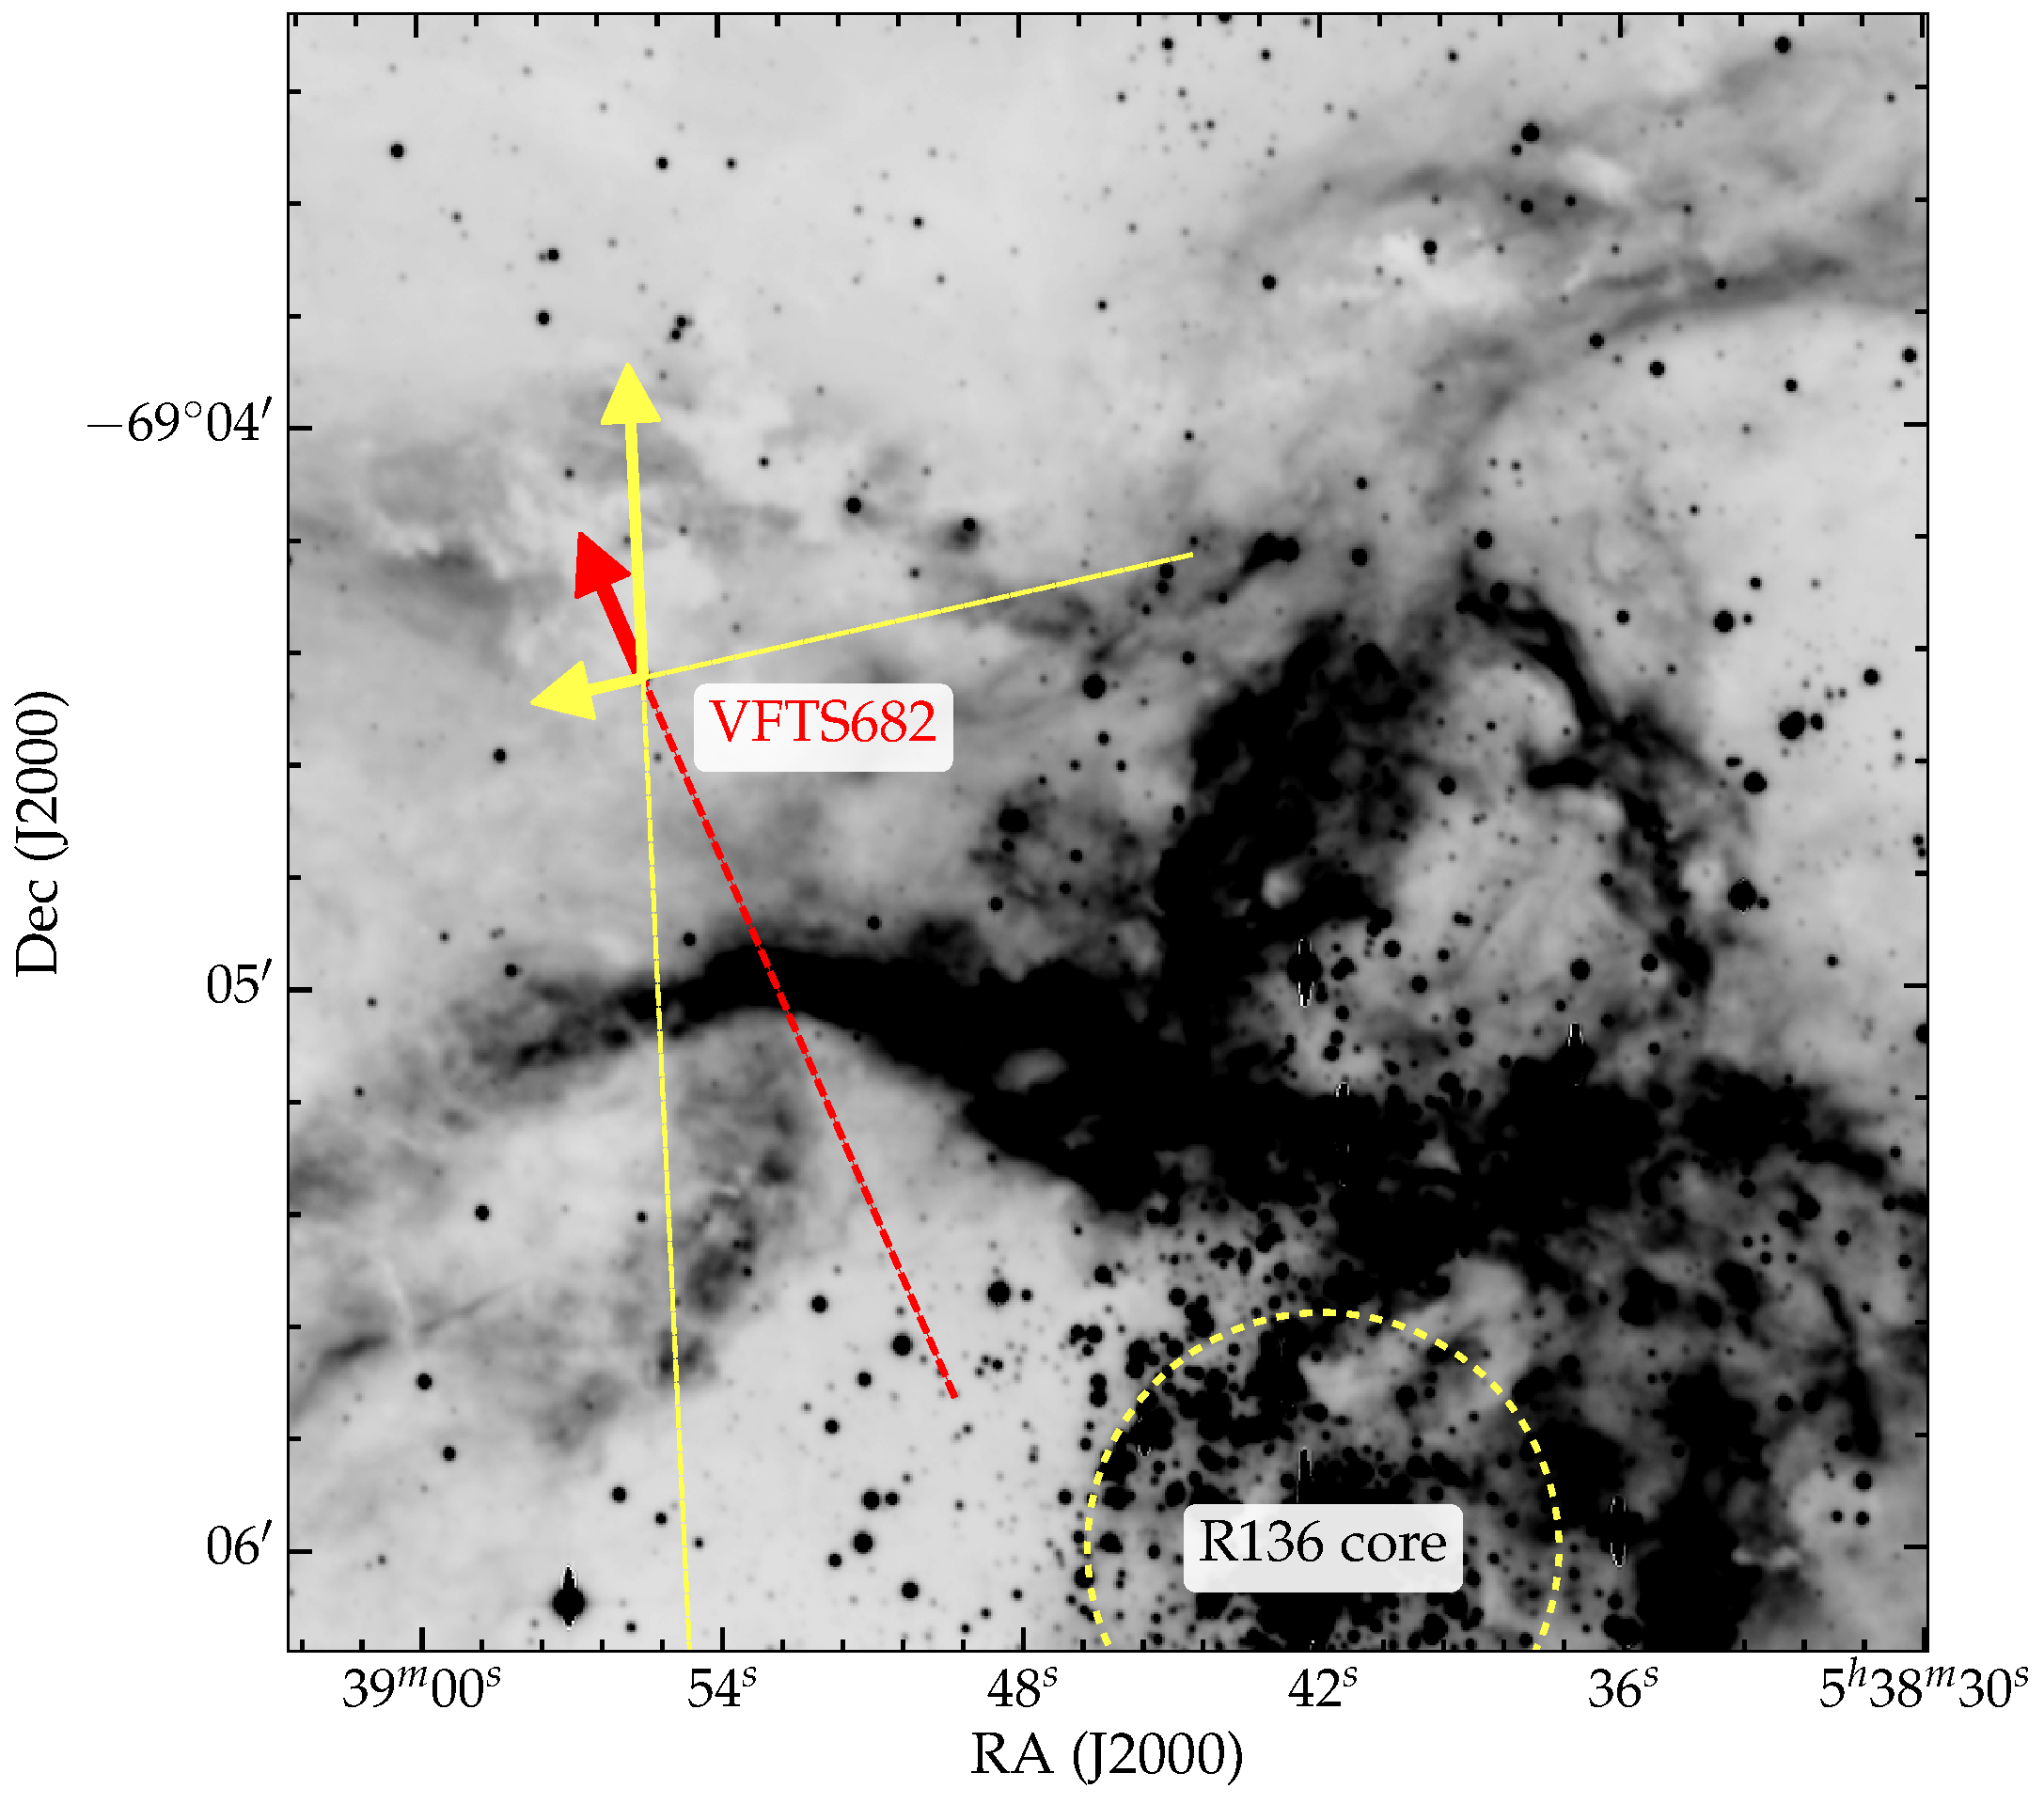
\includegraphics[width=0.48\textwidth]{./figures/main_plot_good_gaia_only}  
  \caption{The red solid arrow indicates the proper motion of VFTS682
    relative to the region from \emph{Gaia} DR2, starting from the present day position of
    the star. The yellow arrows indicate the possible
    directions of projected motion within the \emph{Gaia} DR2 errors, and are extended
    backwards (dashed) to illustrate the uncertainty on the origin of the
    star. The length of the prolongations is proportional to the relative proper motion
    times the age of VFTS682 \citep[$1.0\pm0.2$\,Myr,][]{schneider:18}.
    % \todo{load color picture on background? Fig with HST data
    % available, but confusing...}
  }
  
  \label{fig:main}
\end{figure}


\section{Discussion}
\label{sec:discussion}

Based on our results, we tentatively claim that VFTS682 is the most massive
runaway known to date, with a peculiar three-dimensional speed of
$44\pm21\,\kms$. Due to the large error bars, this result will need
to be revisited with future astrometric data. % to be revisited as updated
% astrometric parameters from future \emph{Gaia} data releases become
% available.
If confirmed, it means that isolated star formation is
\emph{not} required to explain the isolation of VFTS682. Its proper motion suggests that it was ejected from the cluster R136
$0.9\pm0.6$\,Myr ago. Because of the exceptionally large mass
of this star, this raises the question of which stars must populate
the core of the cluster.

Dynamical ejections due to N-body interactions typically (although, not necessarily) eject the least
massive star among those interacting \cite[e.g.,][]{banerjee:12}. This means that, just
based on the kinematic properties of VFTS682, we would expect several
stars with initial masses larger than $\sim$$150\,M_\odot$ in the
cluster R136.
This is consistent with the detection
of extremely massive stars in the core of the
cluster. % The projected rotational equatorial
% velocity\footnote{However, the determination of the rotational
%   velocity for stars showing lines in emission is complicated by the optically thick wind screening the surface of the star, and should be
%   considered with caution.} of VFTS682
% reported by \cite{schneider:18} is $v\sin(i)<200\,\kms$, which is in
% line with the average rotation rate of massive stars in the region
% \citep[][]{ramirez-agudelo:15}. This suggests that VFTS682 (i) has not
% experienced rotationally induced chemically homogeneous evolution
% \citep[][]{maeder:00,demink:09}, and (ii) it has not
% accreted mass from or merged with a binary companion, nor will it, since the multi-epoch
% data of the VFTS survey rule out the presence of a close companion at the
% present day. Moreover,

The spectral type of VFTS682
\citep[WNh5,][]{bestenlehner:11} is the same as R136a1-a3, i.e.~the
three most massive stars detected in the core of the cluster%  by
% \cite{dekoter:97,crowther:10,crowther:16}
, with an astonishing similarity in particular with
the spectrum of R136a3. Therefore, the isolation of
VFTS682 makes it an ideal target to constrain the stellar physics of
stars with masses well above $\sim$$100\,M_\odot$ while avoiding
crowding issues. %  : its isolation makes
% it an easier target for observations compared to the similar stars
% present in the crowded core of R136.

\citet{banerjee:12} used N-body simulations of fully segregated
clusters with all massive stars in binaries to suggest that VFTS682
was ejected from R136. They
demonstrated that the cluster potential does not significantly change
the velocity of the star after the ejection. In their
model, they relied on (dynamically driven) stellar mergers to explain the high masses of
VFTS682 and the massive members of R136.%  While it is not possible to
% robustly exclude that VFTS682 is itself a merger, its spectrum does not show any of the obvious signatures
% like fast rotation, which however could have already slowed down
% because of the wind angular momentum losses during and after the
% merger.

To eject such a massive object, the cluster is
expected to have produced
a large number of massive runaways. Indeed, several %relatively
isolated massive stars are observed in the region, some with known
large radial velocities and/or proper motion. % (see
% \Figref{fig:pm_polar} and Sana et al., in prep.).
A comprehensive study of the kinematic
properties of all the massive stars surrounding R136 might shed light
on whether some can be unequivocally identified as merger products. It
is also possible that the star or binary that caused the ejection of
VFTS682 might have been ejected in the opposite direction, and is also
isolated at present day. If the ejection was caused by an interaction
with a binary, however, it is likely that the binary scattered in the
opposite direction will experience further dynamical interactions on
its way, modifying its trajectory and making it difficult to find.  %absence of proof would not undermine our conclusions 

The similarities between VFTS682 and the WNh5 stars in the core of
R136 are also in agreement with the ``bully binary'' model of
\cite{fujii:11}. Based on their numerical results, they suggested that
early in the evolution of a cluster, dynamical interactions form an extremely
massive binary, which then tightens its orbit by ejecting other stars passing
by. Interpreting our results for VFTS682 through the lens of their simulations
suggests the presence of a close binary with total mass
$M_1+M_2\gtrsim 300\,M_\odot$ in the core of the cluster. Such bully
binary could be R145 according to \cite{fujii:11}, and it might be an
ideal observational candidate for a dynamically formed progenitor system of
a binary black-hole, provided that stars this massive can avoid a
pair-instability supernova \cite[e.g.,][]{rakavy:67} at LMC
metallicity \citep[see also][]{langer:07}. Similarly, the final fate of VFTS682 could be either a
pair-instability supernova without compact remnant formation, or
possibly direct collapse to a black hole above the $2^\mathrm{nd}$
mass gap. The amount of mass loss of these stars will determine their final core
mass and thus their final fate.

The kinematic age of VFTS682 puts an
upper limit to the timescale to form the ``bully binary'' in
R136. The cluster must have been at the very beginning of its
evolution, given the age estimate of $\lesssim 2$\,Myr
\citep[][]{crowther:10,sabbi:12} and the kinematic age of VFTS682. If the
cluster is indeed younger than the shortest stellar lifetime
\citep[$\sim$3\,Myr, e.g.,][]{brott:11, zapartas:17}, then the alternative
explanation for ejection of VFTS682 from the disruption of a binary
by a core-collapse event is excluded since the region is too young for stars
to have experienced core-collapse already.

The variability of VFTS682, reminiscent of LBV stars, suggests
that VFTS682 (and therefore its analogs in the core of R136) might
experience enhanced mass loss episodes in LBV eruptions. \citet{smith:15} made the highly
debated\footnote{See, e.g., \cite{humphreys:16, davidson:16, smith:16}.}
claim that LBV stars are typically isolated form O-type stars. The fact that VFTS682 is a dynamically
ejected runaway which might evolve into an LBV star suggests that
N-body interactions also play a role in explaining the apparent
isolation of at least some LBV stars. 

\todo{maybe move around fig. 1
\message{ !name(VFTS682_APJL.tex) !offset(844) }

\end{document}




%%% Local Variables:
%%% mode: latex
%%% TeX-master: t
%%% End:
